%ドキュメントスタイルの設定
\documentclass[12pt]{jsarticle} %文字サイズ12pt

%引用スタイルの設定
\bibliographystyle{junsrt}

%パッケージ(ここは各自の使いたいパッケージをもってくる)
\usepackage[dvipdfmx]{graphicx}
\usepackage[dvipdfmx]{color}
\usepackage{here}
\usepackage{dcolumn}
\usepackage{multicol}
\usepackage{graphicx}
\usepackage{longtable}
\usepackage{url}
\usepackage{amssymb}
\usepackage{multirow}

%本文の文字数,行数の定義
\setlength{\textwidth}{37zw} %本文の幅 %1行37文字
\setlength{\textheight}{36\baselineskip} %本文の高さ %1ページ36行

%余白の定義
\setlength{\hoffset}{0.5cm} %出力位置の調整(横) %0.5cm右にずらす
\setlength{\voffset}{0cm} %出力位置の調整(縦)
\setlength{\topmargin}{0cm} %ページ上端の余白
\setlength{\headheight}{0cm} %ヘッダ領域の高さ
\setlength{\headsep}{0cm} %ヘッダ領域下端と本文領域上端の間隔

%図番号の定義
\makeatletter
\@addtoreset{figure}{section}
\def\thefigure{\thesection.\arabic{figure}} %章番号.英数字(1~)の形
\makeatother

%表番号の定義
\makeatletter
\@addtoreset{table}{section}
\def\thetable{\thesection.\arabic{table}} %章番号.英数字(1~)の形
\makeatother

%数式番号の定義
\makeatletter
\@addtoreset{equation}{section}
\def\theequation{\thesection.\arabic{equation}} %章番号.英数字(1~)の形
\makeatother

%表紙の記載する内容の定義
\makeatletter
\def\@thesis{2021年度卒業論文}
\def\id#1{\def\@id{#1}}
\def\department#1{\def\@department{#1}}
\title{マイコンと汎用センサーを用いた安価なリアルタイム呼吸代謝測定装置の製作} %タイトル
\date{\today} %日付
\department{環境情報学部} %学部
\id{71741818} %学籍番号
\author{尾島航基} %名前
\makeatother

%表紙の組版
\makeatletter
\def\@maketitle{
\begin{center}
{\huge \@thesis \par} %修士論文と記載される部分
\vspace{50mm}
{\LARGE\bf \@title \par} %論文のタイトル部分
\vspace{30mm}
{\Large \@date\par} %提出年月日部分
\vspace{50mm}
{\Large \@department \par} %所属部分
{\Large 学籍番号 \@id \par} %学籍番号部分
\vspace{10mm}
{\Large \@author} %氏名
\end{center}
\par\vskip 1.5em
}
\makeatother

\newcommand{\ifdraft}{false} %分割したファイルを読み込むための仕掛け

%ここまでヘッダー

%ここから論文作成の開始
\begin{document}
%表紙
\maketitle %表紙の作成
\thispagestyle{empty} %ページ番号なし
\newpage %改行
\addtocounter{page}{-1} %ページカウントを0にする

%論文要旨
\thispagestyle{empty} %ページ番号なし
\expandafter\ifx\csname ifdraft\endcsname\relax
 \begin{document}
\fi

\section*{卒業論文 2021年度(令和3年度)\\汎用センサーを用いた呼吸代謝測定装置の自作}
\subsection*{論文要旨}
\noindent %先頭を改行しないという指示
%ここに論文要旨を書く.

現在,スポーツ中の各種データを取得できるデバイスはアマチュアレベルでも広く普及しているが,呼気分析によって得られるデータを取得できるデバイスは普及しているとは言いがたい.呼気分析によって最大酸素摂取量(\.{V}_{O_2max})や消費エネルギーの高精度な推定など,より有用なデータの取得が可能になる.本研究では入手性が高い安価な汎用センサーを用いて,個人レベルで利用できる呼気分析を行うことができるデバイス(呼吸代謝測定装置)を製作し,その精度や有用性を検証する.

\\
\\
キーワード\\
1.センサー 2.呼気分析 3.インドアスポーツ 4.呼吸代謝測定装置 5.マイコン\\
\begin{flushright} %右寄せをするという指示
  慶應義塾大学 環境情報学部\\
  尾島航基
\end{flushright}

\expandafter\ifx\csname ifdraft\endcsname\relax
  \end{document}
\fi

\newpage %改行
\addtocounter{page}{-1} %ページカウントを0にする

%目次
\pagenumbering{roman} %ページ番号のスタイル
\tableofcontents %目次の作成
\newpage %改行
\addtocounter{page}{-1} %ページカウントを0にする

%本文開始
\pagenumbering{arabic} %ページ番号のスタイル


%各章ごとに分割したファイルの読み込み
%\expandafter\ifx\csname ifdraft\endcsname\relax
 \begin{document}
\fi

\section{章}
\subsection{節}
texで卒業論文を書く時のテンプレートを作成した.構成は,以下の通り.
\begin{enumerate}
  \item 表紙
  \item 論文要旨
  \item 目次
  \item 典型的な章(使い回す)
  \item 参考文献
  \item 謝辞
\end{enumerate}

\subsection{表のテンプレート}
表のテンプレートを以下に示す(表\ref{tb:table_temp}).
\begin{table}[H]
  \begin{center}
   \caption{表のテンプレート}
    \label{tb:table_temp}
    \begin{tabular}{|c||c|} 
\hline
a & b  \\ \hline \hline
 	01 & 02   \\ \hline
	03 & 04   \\ \hline
    \end{tabular}
  \end{center}
\end{table}

\subsection{数式のテンプレート}
数式のテンプレートを以下に示す(式\ref{math_temp01}).
\begin{eqnarray}
\label{math_temp01}
  \mbox{\boldmath $F$} = m\mbox{\boldmath $a$}
\end{eqnarray}

数式が数行にわたる場合は以下の通り(式\ref{math_temp02}).
\begin{eqnarray}
\label{math_temp02}
  \mbox{\boldmath $\ddot{x}$} &=& \frac{\mathrm{d^2}\mbox{\boldmath $x$}}{\mathrm{d}t^2} \nonumber \\
  &=& \frac{\mathrm{d}\mbox{\boldmath $v$}}{\mathrm{d}t}
\end{eqnarray}

\subsection{引用のテンプレート}
参考にしたサイトは脇田\cite{tex_ref02}や山本\cite{tex_ref01}など.\par

\subsection{画像のテンプレート}
tempフォルダ以下のファイルの構成を以下に示す(図\ref{fig:img_temp}).
\begin{figure}[H]
  \begin{center}
    \includegraphics[keepaspectratio, scale=0.2]{../Fig/img_temp.png}
    \caption{tempフォルダ以下ののファイルの構成}
    \label{fig:img_temp}
  \end{center}
\end{figure}

\expandafter\ifx\csname ifdraft\endcsname\relax
  \end{document}
\fi

\expandafter\ifx\csname ifdraft\endcsname\relax
 \begin{document}
\fi

\section{緒言}

\subsection{スポーツセンシングの現状}

近年,小型軽量かつ安価なウェアラブルデバイスでスポーツ中の様々なデータをリアルタイムに測定・記録することが可能になった.特に持久系スポーツにおいては,激しい動きが少なく運動中の測定が行いやすいことから,現在では様々なデータを記録し、トレーニングに活用することが普及している.例として,ランニングやサイクリングにおける,GPSを用いた移動距離やスピードの測定や,ランニングやスイミングにおける加速度センサーなどを用いたフォームの分析,サイクリングにおける歪みセンサーを用いたパワー測定など,現在私たちがリアルタイムに測定が可能な項目は非常に多岐にわたる.

\subsection{呼気分析の現状}

一方で,研究室レベルでは古くから行われてきた呼気分析によって得られる各種データを測定するデバイスは,個人レベルで使用できる安価なものが普及するには至っていない.それにも関わらず,酸素摂取量を推定することによって得られる最大酸素摂取量や運動強度,消費エネルギーの推定などの指標は多くの人々が利用するデバイスで多くの人が利用するという状況になっている.酸素摂取量などの呼気分析が現在普及しているデバイスのように気軽に利用できるようになれば,そのデータをより効率的なトレーニングや安全な運動に役立てることが可能になるだろう.そこで,本研究では個人レベルで利用できる呼気分析を行うことができるデバイス(呼吸代謝測定装置)を,安価なマイコンと汎用センサーを用いて製作する.

また,2019年に出現し現在も世界中で猛威を振るっているCOVID-19によって,スポーツの在り方も変化を受けている.大人数で集まって行うようなトレーニングが行えなくなったほか,自宅などに居ながらにしてインターネット経由で世界中の人々と競技ができるインドアスポーツは急速な盛り上がりを見せている.移動を伴わないインドアスポーツはスポーツセンシングとの相性も良く,呼気分析の需要も今後高まっていくことだろう.本研究は,そのような新たなスポーツの在り方に役立つ新たなデバイスを製作することを目的とする.

\subsection{既存の呼吸代謝測定装置}

参考までに,現在日本で購入が可能な呼吸代謝装置とその価格を示す.以下の製品はいずれも株式会社フォーアシストが国内で販売している製品で,価格は同スアの税抜販売価格である.

\begin{table}[]
\begin{center}
  \caption{既存の呼吸代謝測定装置}
  \label{tb:existing_rmmd}
  \begin{tabular}{|l|l|l|}
  \hline
  製品名              & 備考              & 価格          \\ \hline
  VO2Master        & マスク型デバイスのみで使用可能 & ¥1,280,000- \\ \hline
  Cardio Coach PRO & ミキシングチャンバーが必要   & ¥4,200,000- \\ \hline
  Cardio Coach MAX & ミキシングチャンバーが必要   & ¥3,600,000- \\ \hline
  MetaCheck        & 安静時代謝測定用        & ¥1,300,000- \\ \hline
  \end{tabular}
\end{center}
\end{table}

\subsection{本研究の目標}

今回製作する装置は,呼気分析による呼吸代謝の測定を小型のマイコン本体のみで行い,測定したデータの記録・表示までをその場で確認できるものとする.これをリアルタイムでの呼吸代謝測定とし,この機能を備えた装置を製作することを目指す.

また,装置本体の価格は,表\ref{tb:existing_rmmd}に見られるような既存の装置の100分の1程度を目標とする.


\expandafter\ifx\csname ifdraft\endcsname\relax
  \end{document}
\fi

\expandafter\ifx\csname ifdraft\endcsname\relax
 \begin{document}
\fi

\section{方法}
\label{sec:method}

\subsection{直接法と間接法}

\subsubsection{直接法}

人体で消費されたエネルギーは熱となって放射される.その熱量を直接測るのが直接法である.例えば,直接法の測定機器であるAtwater-Benedict-Rosa calorimeterでは,測定室内の被験者が放射する熱を室内に張り巡らされた管を流れる水の温度から測定する.それに加え,室内で発生した水蒸気量呼気などの水蒸気の気化熱を測定するとともに,測定中の体温の変化も考慮して,被験者のエネルギー消費量を測定する\cite{tanaka_2006}.

このように装置が大掛かりで,活動内容も測定室内で行えるものに限られるため,現在でも使用は一部の実験施設などに限られている.

\subsubsection{間接法}

そこで,測定が容易な別の値から間接的に消費エネルギーを求める方法が考案されてきた.中でも心拍数を用いて消費エネルギーを推定する方法は古くからRMR法などの方法が用いられ\cite{usutani_1990},現在では様々なデバイスやサービスで利用することができる.

しかし,心拍数は同一の被験者においても気温や体調によるばらつきが大きく,これを用いた消費エネルギーの推定は精度面で問題が残る.そこで,直接法ほど大掛かりな装置を用いずにより正確に消費エネルギーを推定する方法として,呼気分析によって消費エネルギーを推定する方法がある.

\subsection{Weirの式}
人体がエネルギーを生み出す際の化学反応から消費エネルギーを推定することができる.食物から取り込んだ栄養素が酸素と反応し,二酸化炭素を産出する.この化学式を用いて,酸素摂取量と二酸化炭素摂取量,尿素窒素量が正確に得られれば,エネルギー消費量が1\%もしくはそれ以下の誤差で推定できる\cite{livesey_1988}.

例えば,よく利用されるWeir\cite{weir_1949}の式は以下の通りである.

\begin{equation}
  \label{weir_urea_formula}
  EE(kcal) = 3.941 \times 酸素摂取量 + 二酸化炭素産生量 - 2.17 \times 尿中窒素排出量
\end{equation}

このうち,尿素窒素排出量は摂取エネルギーに閉めるたんぱく質の割合によって決まる.この値は比較的安定しており,たんぱく質の占める割合を12.5\%と仮定するとWeirの式は次のようになる.

\begin{equation}
  \label{weir_formula}
  EE(kcal) = 3.9 \times 酸素摂取量 + 1.1 \times 二酸化炭素産生量
\end{equation}

尿中窒素排出量を使用しないWeirの式は,たんぱく質の占める割合が20\%を大きく超えるような極端に偏った食事や,激しい運動中に限定したりすることをしなければ,誤差の影響は1\%未満であり,酸素摂取量と二酸化炭素産出量のみでも十分に正確に測定することができる\cite{tanaka_2006}.

呼気分析とWeirの式を用いた間接法は,直接法に比べて実施が容易である上に,心拍数などを用いた場合に比べてより精度の高い推定が可能である.それに加えて,呼気分析によって得られる酸素摂取量(VO2),呼吸回数(RR)及び換気量(VE)などの値は,アマチュアアスリートにとってもトレーニングや安全な運動のために有用なデータとなりうる.そこで,今回は呼気分析によって消費エネルギーを測定することができる呼吸代謝測定装置を製作する.

\subsection{計測項目}

\subsubsection{酸素摂取量(\.{V}_{O_2})と二酸化炭素産出量(\.{V}_{CO_2}),呼吸商}

酸素摂取量\.{V}_{O_2}は空気中の酸素(O_2)が単位時間(今回は慣例に従い1分間値とする)あたりにどれだけ身体に採り入れられたかを表す値である.よって,身体(肺)に採り入れた空気の量の大きさ(肺換気量)と吸気ガスと呼気ガスの酸素濃度の差(酸素の減少率)によって\.{V}_{O_2}を求めることができる.吸気中に含まれる窒素は身体内に入らないため,この分を補正して酸素摂取量を求める.吸気の酸素分圧をF_{IO_2},吸気の(大気中)二酸化炭素分圧をF_{ICO_2},呼気の酸素分圧F_{EO_2},呼気の二酸化炭素分圧F_{ECO_2}とすると,酸素摂取量\.{V}_{O_2}は次のように表せる.

\begin{equation}
  \.{V}_{O_2} = V_E \frac{ 1 - F_{EO_2} - F_{ECO_2} }{ ( 1 - F_{IO_2} - F_{ICO_2} ) \times F_{IO_2} - F_{EO_2} }
\end{equation}

このうち大気中の二酸化炭素F_{ICO_2}(0.003\%)は十分に小さいことから無視できるとし,\.{V}_{O_2}は次のようになる.

\begin{equation}
  \.{V}_{O_2} = V_E \frac{ F_{IO_2} - F_{EO_2} - F_{ECO_2}F_{IO_2} - F_{IO_2}F_{EO_2}}{ 1 - F_{IO_2}}
\end{equation}

同様に,二酸化炭素産出量\.{V}_{CO_2}は次のように表される.

\begin{equation}
  \.{V}_{CO_2} = V_E F_{EO_2}
\end{equation}

また,これらから単位時間あたりに消費される酸素量と二酸化炭素産生量の比である呼吸商(RQ)が求められる.

\begin{equation}
  RQ = \frac{ \.{V}_{O_2} }{ \.{V}_{CO_2} }
\end{equation}

\subsubsection{脂肪燃焼量と炭水化物燃焼量}

\subsection{酸素摂取量(VO_2)}
\label{sec:vo2}

\subsubsection{酸素摂取量の測定の原理}

酸素摂取量VO_2は空気中の酸素(O_2)が単位時間(今回は慣例に従い1分間値とする)あたりにどれだけ身体の中に採り入れられたかを表す値である.よって,VO_2は吸気量V_Iと吸気中の酸素濃度F_IO_2の積(吸気中酸素量)から,呼気量V_Eと呼気中の酸素濃度F_EO_2の積(呼気中酸素量)を引いたものとして求めることができる(図\ref{fig:vo2_measurement_mechanism}).

\begin{equation}
  \label{eq:vo2fife}
  VO_2 = (V_I \times F_IO_2) - (V_E \times F_EO_2)
\end{equation}

\begin{figure}[h]
  \begin{center}
    \label{fig:vo2_measurement_mechanism}
    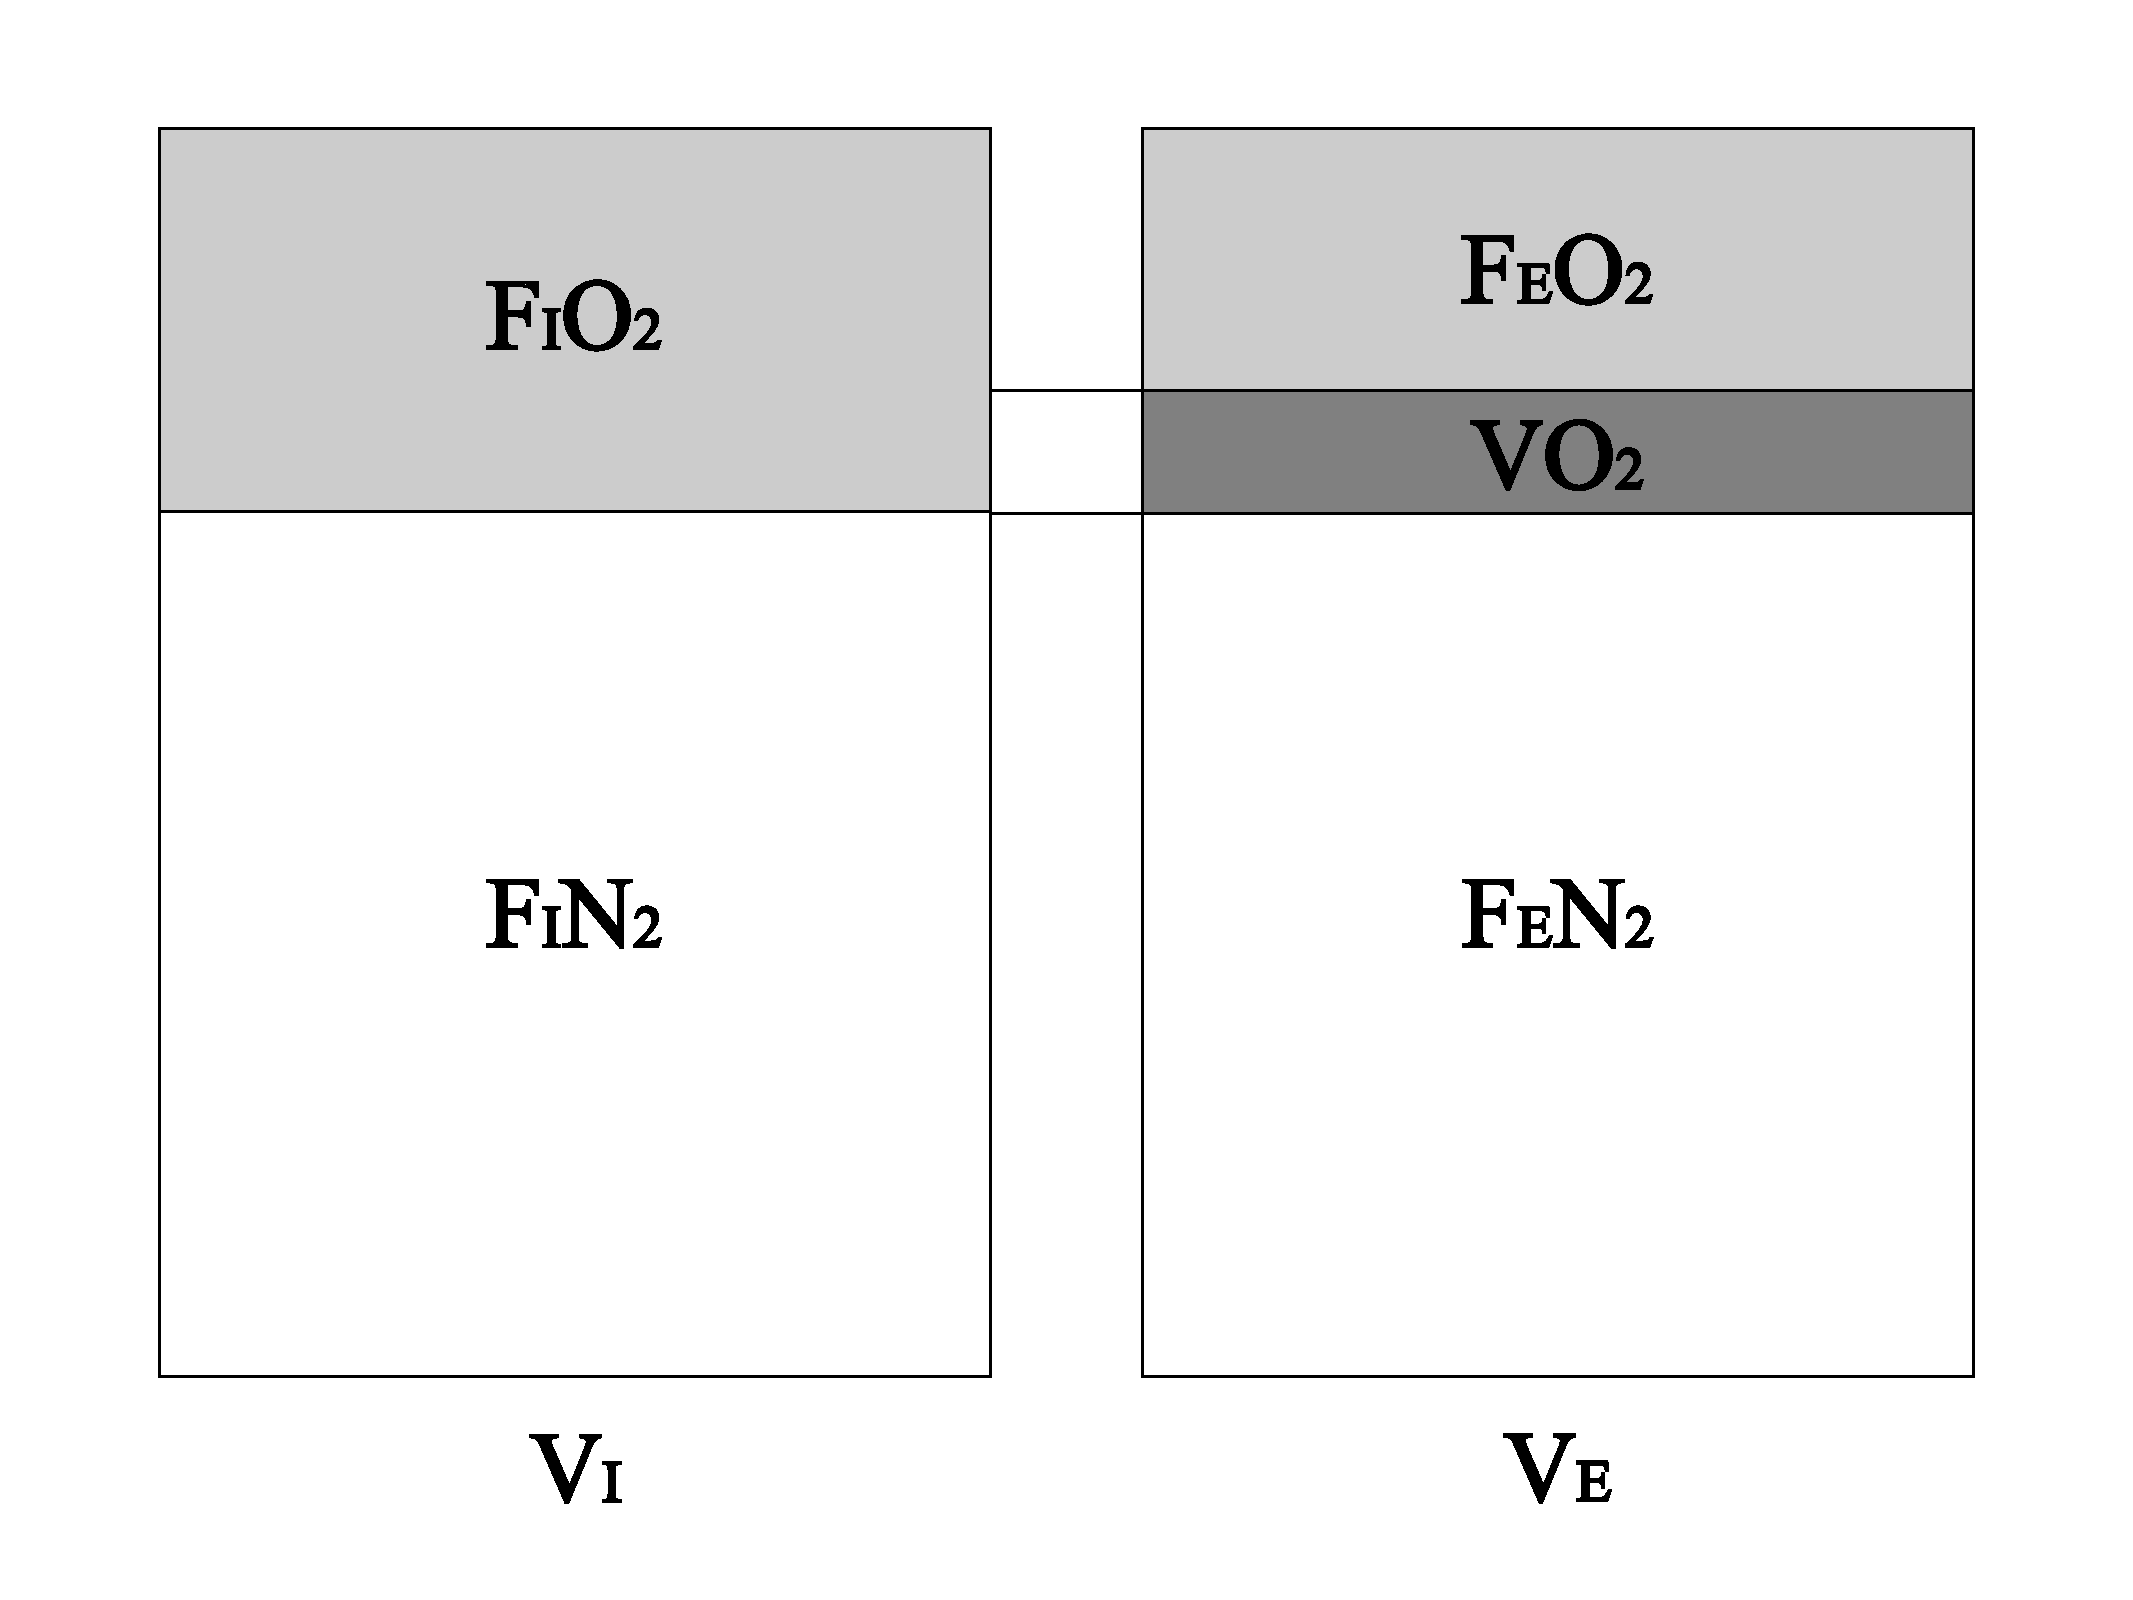
\includegraphics[width=5cm]{fig/vo2_measurement_mechanism.pdf}
    \caption{VO_2の測定}
  \end{center}
\end{figure}

このうち,吸気量V_Iは直接測定しなくても,吸気中および呼気中の窒素量から求めることが可能である.\ref{sec:n2correction}で解説する.

\subsubsection{窒素補正}
\label{sec:n2correction}

窒素は代謝に使われないため体内に吸収されない.そのため,吸気中と呼気中の窒素量は変わらないという特性を持つ(図\ref{fig:vo2_measurement_mechanism}).これを利用することで,吸気量V_Iを直接測定せずに求めることが可能である.
吸気中及び呼気中の窒素量は,吸気量または呼気量に,それぞれ吸気中の窒素濃度F_IN_2,呼気中の窒素濃度F_EN_2を掛けたものとして求められる.これと先述の窒素の特性を用いて,次の式が成り立つ.

\begin{equation}
  \label{eq:fin2fen2}
  V_I \times F_IN_2 = V_E \times F_EN_2
\end{equation}

また,この特性から呼気中の窒素濃度は,呼気中の酸素濃度F_EO_2と二酸化炭素濃度F_ECO_2を100\%から引いた残りであると考えられるから,次の式が成り立つ.

\begin{equation}
  F_EN_2 = 100 - F_EO_2 - F_ECO_2
\end{equation}

式\ref{eq:fin2fen2}をV_Iに関して変形すると

\begin{equation}
  \label{eq:vefin2fen2}
  V_I = \frac{V_E \times F_EN_2}{F_IN_2}
\end{equation}

式\ref{eq:vefin2fen2}を式\ref{eq:vo2fife}に代入すると

\begin{equation}
  \label{eq:vo2ve}
  VO_2 = \underbrace{\frac{V_E \times F_EN_2}{F_IN_2} \times F_IO_2}_{吸気中酸素量} - \underbrace{V_E \times F_EO_2}_{呼気中酸素量}
\end{equation}

式\ref{eq:vo2ve}の右辺のV_Eを括り出して整理すると

\begin{equation}
  \label{eq:n2correctformura}
  \underbrace{VO_2}_{酸素摂取量} = \underbrace{V_E}_{呼気量} \times \underbrace{\overbrace{( \frac{F_EN_2}{F_IN_2} \times F_IO_2 - F_EO_2 )}^{窒素補正}}_{酸素摂取量}
\end{equation}

式\ref{eq:n2correctformura}では,窒素は代謝に使われないため吸気中と呼気中の窒素量は変わらないという特性を利用して,吸気中の酸素濃度を呼気量に相当した酸素濃度に換算している.これを窒素補正という.

右項の酸素摂取率は,窒素補正された呼気ガス量に対する酸素濃度から,呼気中の酸素濃度を引いて得られる.
呼気中の窒素濃度は,呼気中の酸素濃度F_EO_2と二酸化炭素濃度F_ECO_2を100\%から引いた残りであると考えられるから,それらを代入すると

\begin{equation}
  VO_2 = V_E \times (\frac{100 - F_EO_2 - F_ECO_2}{F_IN_2} \times F_IO_2 - F_EO_2)
\end{equation}

通常大気中(吸気中)の窒素濃度は79.04\%,酸素濃度は20.93\%であるから,これらの値を代入して

\begin{equation}
  VO_2 = V_E \times (\frac{100 - F_EO_2 - F_ECO_2}{79.04} \times 20.93 - F_EO_2)
\end{equation}

\begin{equation}
  VO_2 = V_E \times { {100 - F_EO_2 - F_ECO_2)} \times 0.265 - F_EO_2) }
\end{equation}

以上の式から,呼気の分析から酸素摂取量を求めることができる.

\subsection{換気量(V_E)}

\subsubsection{換気量の測定}

\ref{sec:vo2}で示したように,換気量V_Eを測定するためには呼気量を測れば良い.



\subsubsection{STPD係数}

呼気量から測定される換気量は,ATPS(Ambient Temperature, Pressure, Saturated with water vapor)においての値である.これは計測環境気温,計測環境気圧,水蒸気飽和における値である.VO_2, VCO_2は慣習としてSTPD(Standard Temperature, Pressure, Dry),0℃,1気圧の気体標準状態で表記されるため,ATPSをSTPDに換算する必要がある.この係数をSTPD係数と呼ぶ.STPD係数は以下の式で表される.

\begin{equation}
  \label{eq:stpd}
  STPD = \frac{P_B - P_{H2O}}{760} \times \frac{273.15}{273.15 + T}
\end{equation}

ただし,P_B: 気圧,P_{H2O}: 飽和水蒸気圧(\ref{sec:swvp}で記述する),T: 気温,273.15: 絶対温度である.

\subsubsection{飽和水蒸気圧}
\label{sec:swvp}

飽和水蒸気圧P_{H2O}は温度によって変化し,Tetens(1930)の式を用いて近似値を求めることができる.温度T[℃]の時の飽和水蒸気圧e(T)[mmHg]は次の式で求められる.

\begin{equation}
  e(T) = 6.1078 \times 10 ^ \frac{7.5T}{(T + 237.3)} \times \frac{760}{1013.25}
\end{equation}

\subsubsection{換気量の計算}

VO_2, VCO_2に使用される換気量は1分間値であるので,換気量V_{ATPS}を求めるためには呼気量Vを採気時間T[min]で割る.

\begin{equation}
  V_{ATPS} = \frac{V}{T}
\end{equation}

これにSTPD係数(\ref{eq:stpd})を掛けると換気量V_{STPD}が得られる.

\begin{equation}
  V_{STPD} = V_{ATPS} \times STPD
\end{equation}

式\ref{eq:vo2ve}より,STPD状態の吸気中酸素量V_IO_2から呼気中酸素量V_EO_2を引くことで酸素摂取量VO_2を求めることができる.

STPD状態での呼気中酸素量V_EO_2は呼気中酸素濃度F_EO2から次の式で求める.

\begin{equation}
  V_EO_2 = V_{STPD} \times \frac{F_EO2}{100}
\end{equation}

章\ref{sec:n2correction}で述べたとおり,吸気中と呼気中の窒素量は変化しない.これを利用して吸気中の窒素量からSTPD状態での吸気中酸素量V_IO_2を次の式から求める.

\begin{equation}
  V_IO_2 = V_{STPD} \times \frac{F_EN_2}{79.04} \times \frac{20.93}{100}
\end{equation}

ただし,79.04, 20.93はそれぞれ通常大気中(吸気中)の窒素濃度は79.04\%,酸素濃度は20.93\%である.

窒素補正を利用し,F_EN_2に代入すると次のようになる.

\begin{equation}
  V_IO_2 = V_{STPD} \times \frac{100 - F_EO_2 - F_ECO_2}{79.04} \times \frac{20.93}{100}
\end{equation}

通常大気中(吸気中)の窒素濃度は79.04\%,酸素濃度は20.93\%であるから,これらの値を代入して

\begin{equation}
  V_IO_2 = V_{STPD} \times \frac{100 - F_EO_2 - F_ECO_2}{79.04} \times \frac{20.93}{100}
\end{equation}

\expandafter\ifx\csname ifdraft\endcsname\relax
  \end{document}
\fi

\expandafter\ifx\csname ifdraft\endcsname\relax
 \begin{document}
\fi

\section{製作}

\subsection{マスク}

\subsubsection{呼気収集マスク}

呼気収集マスクには,仰木研究室内で以前に製作されたマスクを使用した.このマスクは,アクリル板を組み合わせて顔に合うような形状を構成し,吸気及び呼気用の通気口を設けた物である.顔に当たる部分にはウレタンフォーム製のクッションを取り付け,頭に取り付けられるように市販のガスマスクから流用したバンドが取り付けてある.

\subsubsection{逆止弁}

\subsection{換気量V_Eの計測}

\subsubsection{計測方式}

換気量V_Eを計測するための流量計には,マイコン工作用として市販されている水流計を使用した.

気体の流量を計測するための流量計の原理としては,差圧流量計と超音波流量計,タービン流量計などがある.差圧流量計は流路内に絞り機構を設け,その前後に発生する圧力差を測ることで流量を計測する方式である.超音波流量計は,流路内を流れる流体に超音波を照射することで流量を計測する方式である.タービン流量計は,流路にタービンを設置し,流体によって回転するタービンの回転数によって流量を計測する方式である.タービン流量計は単純な構造であり,他の方式に比べて微細ではない構造なので,水流計として安価に市販されている.呼吸代謝測定装置のうち,流量計は高価な部品であり,全体の価格を抑えるためにタービン流量計を使用した.

今回使用した流量計はYF-S201という名称で販売されているもので,流路に対してタービンの軸が垂直に取り付けられている接線流羽根車式のタービン流量計である.タービンの回転数に応じてホール素子が矩形波の信号を出力する.主な仕様を表\ref{tb:YFS201_specsheet}に示す.

\begin{table}[h]
  \begin{center}
  \caption{YF-S201 主な公称仕様}
  \label{tb:YFS201_specsheet}
    \begin{tabular}{lc}
      流路外径 & 20mm \\
      入口内径 & 9mm \\
      出口内径 & 12mm \\
      動作流量 & 1-30L/min \\
      関係式 & 1L_{水} = 450pulse
    \end{tabular}
  \end{center}
\end{table}

\subsubsection{タービン式水流計の流量関係式の算出}

仕様によれば,YF-S201は水流1Lあたりに450個の矩形波を出力する.これは水流が流れる時の値なので,空気の流量計として使用するためには空気が流れる際の関係式を求める必要がある.今回はこれを実験で求めた.

\begin{figure}[h]
  \begin{center}
    \label{fig:flowsensor_calibrate}
    \includegraphics[width=8cm]{fig/flowsensor_calibrate.png}
    \caption{流量関係式算出用の実験}
  \end{center}
\end{figure}

図\ref{fig:flowsensor_calibrate}は実験の全景である.
空気の量を正確に測りとれるシリンジを流量計の入り口に接続し,一定量の空気を送り込んだ時のタービンの回転数,すなわち矩形波の数を計測した.
送り込む空気の量は,入手が可能であったシリンジの最大サイズから300mLとした.シリンジのピストンを押す速さが出来る限り一定になるように注意しながら手でピストンを押した.シリンジと流量計の接続部は空気が漏れないようにするためにジョイント部品を製作した.シリンジのノズルと流量計のネジ部分を接続する部品を3Dプリンターで製作した.また,予備実験において,シリンジのノズルから出た高圧の空気が流量計のタービンの羽根に直撃すると回転数が多くなることが確認できたため,図\ref{fig:syringe_cone}のように,ノズルから出た空気が一度中央に当たってから流量計へと流れる形状とした.

\begin{figure}[h]
  \begin{center}
    \label{fig:syringe_cone}
    \includegraphics[width=8cm]{fig/syringe_cone}
    \caption{シリンジと流量計の接続用ジョイント部品}
  \end{center}
\end{figure}

今回使用した流量計はタービン軸の回転の滑らかさが重力に影響されやすいことが予備実験から分かった.そこで,流量計の角度を実際にマスクに取り付けた際の顔を正面に向けた場合を想定し,60度に保持するための治具を3Dプリンターで製作した.
今回の装置では流量計は呼気側の逆止弁の排気側に取り付けられるため,呼気から吸気に切り替わった後も一定時間タービン流量計が空転する.正しく換気量を計測するためにはこの空転分の回転数を除外する必要がある.そこで,回転数を計測するプログラムにこれを除外する処理を加えた.0.1秒毎の回転数を計測し,一個前の区間と比べて値が減少している区間の回転数を除外するという方法で行った.
以上の処理を行い,空転分を除外した回転数を計測するプログラムをM5Stack Core2で動作させ,200回分のデータの代表値を0.3mLの空気が流れた時の回転数とするという方法で流量関係式の算出を行った.結果は以下の通りである.

ミキシングチャンバー方式で換気量を測定するため,マスクの呼気方向にのみ解放される弁の先に取り付けた流量計で換気量を測定する

今回はマイコンなどに接続する水量計として安価に市販されているタービン流量計を流量計に用いた.YF-S201という名称で販売されているもので,タービンの回転数をホール素子センサーによって測定するものである.

呼気のような微小な気体の流量を測定するための流量計には,差圧流量計,超音波流量計,タービン流量計などが用いられる.

差圧流量計は,流路内に絞り機構を設置し,その前後に設置した圧力計から得られる圧力差から流量を測定する方式である.絞り機構としてオリフィスプレートを用いたものはオリフィス流量計と呼ばれる.
超音波流量計は流路内を流れる流体に超音波を照射することで流量を測定する方式である.
タービン流量計は流路にタービンを設置し,流体によって回転するタービンの回転数によって流量を測定する方式である.

%差圧流量計は,流路内に絞り機構を設置し,その前後に設置した圧力計から得られる圧力差から流量を測定する方式である.絞り機構としてオリフィスプレートを用いたもの(オリフィス流量計)はCardioCorchやVO2000などの既存の呼吸代謝測定装置で使用されている.

%超音波流量計は流路内を流れる流体に超音波を照射することで流量を測定する方式である.高精度が特徴であり,NASAが開発したPUMAに使用されている.

既存の呼吸代謝測定装置の流量計には主に先述の三方式が用いられるが,今回は水流センサーとして汎用的に安価に入手が可能であるということでタービン流量計を用いた.

\subsubsection{信号処理}

タービン流量計は流路が気体を流れていない時間も数秒間タービンが空転する.よって,タービンが空転しているだけの時間に測定される流量はデータから除外する必要がある.
YF-S201が出力する信号は高周波のノイズ成分があるため,これをハイパスフィルターを用いて除外する必要がある.今回は計算の容易さからRCフィルターを用いた.

\subsection{酸素センサー}

\subsubsection{空気亜鉛電池式センサー}

今回は株式会社ピーバンドットコムから発売されている「実習用酸素センサキット A-5S」(以下「A-5S」)を酸素センサーとして使用した.A-5Sは,補聴器など用に汎用的に使用される空気亜鉛電池をセンサーとして使用し,空気亜鉛電池の出力電圧から酸素濃度を測定するというセンサーで,組み立てキットとして1000円程度で購入が可能である.構造は単純で空気亜鉛電池に固定抵抗と可変抵抗を接続したというものである.キャリブレーションは大気中の酸素濃度20.84\%とに合わせて出力電圧が20.84mVになるように可変抵抗を調整して行う.空気亜鉛電池の電圧の低下から,長時間連続での測定は困難である.

従来,呼吸代謝測定装置の酸素センサーにはガルバニ電池式センサーが多くの場合で使われてきた.この方式は高精度であるが,酸素濃度に応じて電圧を出力することで酸素濃度を測定するためのガルバニ電池が10000円以上と高価であるため,安価に入手できる空気亜鉛電池をセンサーとして用いたA-5Sを使用した.

\subsubsection{信号処理}

A-5Sが出力する電圧は酸素濃度21\%時に21mVと非常に微弱である.この電圧を今回使用したマイコン,M5Core2(ESP32)の12bit ADコンバーター(0-3.3V, 4096段階)で測定するために,アペアンプを使用して増幅した.オペアンプには,単電源のフルスイングオペアンプNJM2732Dを用いた.非反転増幅回路を用いてA-5Sの出力電圧を101倍に増幅し,酸素濃度21\%時に2.1V程度に増幅することで測定精度を高めている.

(回路図)

\subsection{二酸化炭素センサー}

二酸化炭素濃度を測定するセンサーにはMH-Z19Bを用いた.このセンサーはNDIR方式(非分散型赤外線吸収方式)を用いて二酸化炭素の濃度を測定する.NDIR方式は,それぞれのガスが持つ特有の吸収波長領域を利用し,特定のガスのみを対象ガスに変化を及ぼすことなく濃度を測定することができるガス濃度の測定方式である\cite{whats_ndir}.MH-Z19Bは,NDIR方式の二酸化炭素濃度センサーの中でも2000-5000円程度で比較的容易に入手できるものである.

MH-Z19Bはコマンドを送信することで二酸化炭素濃度をppm単位で容易に取得することが可能である.今回はArduino用のライブラリを用いてppm単位の二酸化炭素濃度を取得し,\%単位に変換してVCO_2の計算に使用している.

\subsection{温度計・湿度計・温度計}

あとでかく.

\subsection{センサー値の計算}

\subsubsection{計算用マイコン}

\subsubsection{プログラム}

\expandafter\ifx\csname ifdraft\endcsname\relax
  \end{document}
\fi

\expandafter\ifx\csname ifdraft\endcsname\relax
 \begin{document}
\fi

\section{検証}

計算の章(\ref{sec:calculation})で述べたように,多くの各種計算値は酸素摂取量VO_2を元に算出される.そこで,今回は実験により運動中の酸素摂取量を測定することによって装置の検証を行う.

酸素摂取量の測定には,トレッドミルや自転車エルゴメーター,踏み台などが用いられる.今回は自宅で実験を行うため,パワーメーター(出力計)を装着したロードバイクを自動負荷調整機能付きのローラー台に取り付けて検証を行った(図\ref{fig:bike_in_use}).
自転車エルゴメーターを使用した酸素摂取量の測定の慣例に従いケイデンス(ペダル回転数)を60rpmに固定した上で,酸素摂取量パワー(出力)をもとに負荷を指定したワークアウトを実行する.ケイデンスを60rpmに固定しているので,パワー(W)を60で割った値が負荷(kp)となる.
ワークアウト中の酸素摂取量に加えて,ロードバイクや身体に取り付けたセンサーによってパワー(W),心拍数(bpm),ケイデンス(rpm)などを測定し,それらの値と酸素摂取量を比較することで装置の有用性について検証する.

\begin{figure}[H]
  \begin{center}
    \includegraphics[width=10cm]{fig/bike_in_use}
    \caption{実験の様子}
    \label{fig:bike_in_use}
  \end{center}
\end{figure}

なお,今回の検証は新型コロナウィルス感染症緊急事態宣言中に行った.呼吸代謝測定装置はマスク部などに唾液が多く付着するため,感染防止の観点から複数人の被験者を対象にした実験を行うことが難しい.よって,実験は筆者が自宅にて自身一人を被験者として行っている.ご了承いただきたい.

%様々な点で装置の検証を行うため,以下の3つの実験を行った.

%\begin{enumerate}
  %\item ランプアップ・ダウン
  %\item 最大酸素摂取量測定
  %\item 負荷変動を伴うワークアウト
%\end{enumerate}

%以上の実験を行った上で,装置が出力するログデータとその他のセンサーで測定したデータをタイムスタンプを用いて統合して検証を行う.

\subsection{実験方法}

最大酸素摂取量(\.{V}O_2Max)以下の低強度で自転車を漕ぐ時,パワーが高いほど酸素摂取量が多くなるはずである.これが実験により確認できるかを検証する.漸増負荷法の定常状態ありの連続負荷法のプロトコルに従い\cite{science_of_vo2},3分ごとに負荷を漸増するという実験を,低強度プロトコルと高強度プロトコル,2種類の設定パワーで行う.それぞれで酸素摂取量を測定し,酸素摂取量とパワー,心拍数を比較することで装置の有効性を検証する.

\subsubsection{実験プロトコル}

酸素摂取量が最大酸素摂取量に近付く高強度の運動では,無酸素系の酸素共有量の不足分(酸素借)を運動を止めた後も有酸素系が補い続けるために安静時よりも酸素摂取量が高い状態が続く.これを酸素負債と呼ぶ.実験に使用する設定パワーは,有酸素系の酸素摂取量のみを見るために,酸素負債が発生しないように出来る限り低強度に設定する.

予備実験から,機材の都合上,ケイデンス60rpmを保ったまま出力できる最低パワーは40W付近であることが分かった.そこで,低強度プロトコルにおける第1段階パワーを40Wとし,高強度プロトコルにおいては30W(ケイデンス60rpm時において0.5kp)増負荷として70Wとした.第1段階パワーからそれぞれ3oW刻みで3分ごとに増負荷とし,設定パワーは表\ref{tb:protocol_power}のようになる.

\begin{table}[]
\begin{center}
  \caption{各プロトコルの設定パワー}
  \label{tb:protocol_power}
  \begin{tabular}{|l|l|l|}
  \hline
       & 低強度プロトコル & 高強度プロトコル \\ \hline
  第1段階 & 40W      & 70W      \\ \hline
  第2段階 & 70W      & 110W     \\ \hline
  第3段階 & 110W     & 140W     \\ \hline
  第4段階 & 140W     & 170W     \\ \hline
  \end{tabular}
\end{center}
\end{table}

本研究で製作した装置は各値の算出に1分平均値を使用しているため,平均値が立ち上がるまでの測定開始後1分間のデータは除外する必要がある.そのため第一段階パワーに入るまでに,40Wでのペダリングをウォーミングアップを兼ねて5分間行い,実際のデータ処理では測定開始後2分後からのデータを用いることとした..以上より,低強度プロトコル,高強度プロトコルはそれぞれ図\ref{fig:protocol_rampup_light},図\ref{fig:protocol_rampup_hard}のようになる.

\begin{figure}[h]
  \begin{center}
    \label{fig:protocol_rampup_light}
    \caption{低強度プロトコル}
    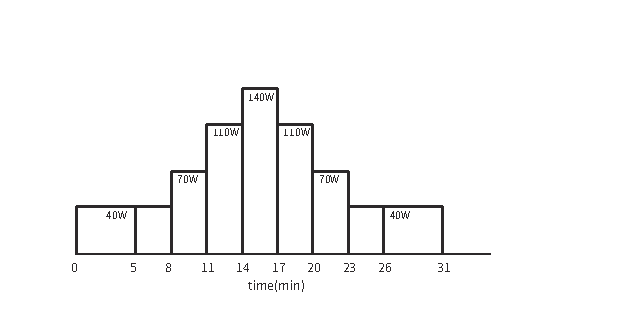
\includegraphics[width=12cm]{fig/protocol_rampup_light.pdf}
  \end{center}
\end{figure}

\begin{figure}[h]
  \begin{center}
    \label{fig:protocol_rampup_hard}
    \caption{高強度プロトコル}
    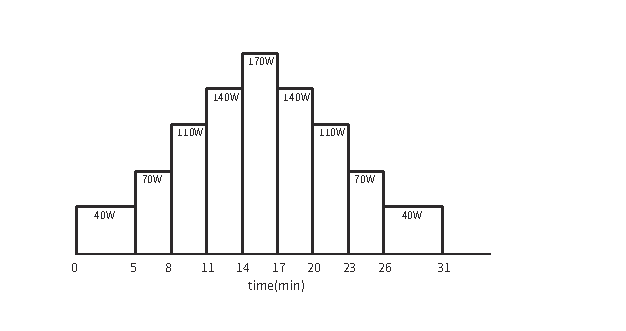
\includegraphics[width=12cm]{fig/protocol_rampup_hard.pdf}
  \end{center}
\end{figure}

\subsection{実験機材}

作成したプロトコルを元に運動を行うためにZwiftのワークアウト機能を用いた.Zwiftはパワーメーター等のパワーソースを接続し,入力されたパワーを元にバーチャルワールド内を自転車に乗ったアバターを操作して走ることができるバーチャルサイクリングプラットフォームである(図\ref{fig:zwift}).Zwiftはパワーや心拍数,ケイデンスなどの走行ログデータが1秒間隔で記録されたFITファイルを保存する.これをmacOS用のユーティリティー,FIT File Explorer\cite{fitfile}を用いてCSVファイルに変換した.

\begin{figure}[h]
  \begin{center}
    \label{fig:zwift}
    \includegraphics[width=8cm]{fig/zwift}
    \caption{Zwiftの実行環境}
  \end{center}
\end{figure}

Zwiftのワークアウト機能はペダリングを開始した時点を0秒とし,その時刻からログデータファイルの記録を開始する.今回製作した装置は1秒間隔でログデータを記録しタイムスタンプを付与する.Zwiftが出力するログデータの記録開始時刻から2分後の時刻を基準とし,両ログデータの同期を行った.

今回使用したパワーメーターは,4iiii InnovationsのPrecision 2.0 3D(図\ref{fig:4iiii})である.自転車運動のパワーを測定する方法は複数あるが,このパワーメーターは左側のクランクアームの裏側に貼り付けた歪みゲージによって計測されたトルクと,加速度センサーによって計測されたケイデンス(ペダル回転数)からパワーを算出する一般的なタイプである.ZwiftとはANT+方式で接続した.

Zwiftが出力するログデータにはPrecision 2.0 3Dが出力する1秒パワーが1秒間隔で記録される.これは変動が大きく, 1分間平均値となる酸素摂取量と比較するのは困難であったため,後処理によって1分平均パワー値を計算して使用した.

\begin{figure}[h]
  \begin{center}
    \label{fig:4iiii}
    \includegraphics[width=8cm]{fig/4iiii}
    \caption{4iiii Innovations Precision 2.0 3D}
  \end{center}
\end{figure}

自動負荷調整機能付きローラー台にはGROWTACのハイブリッド式(前輪固定式)ローラー台のGT-ROLLER Flex3(図\ref{fig:gt-roller_flex3})を用いた.なお,自動負荷調整装置であるGT-ePower-FとGT-eBoxを取り付けているが,今回の実験においては自動負荷調整機能は無効化し最低負荷に固定して使用している.

\begin{figure}[h]
  \begin{center}
    \label{fig:gt-roller_flex3}
    \includegraphics[width=8cm]{fig/gt-roller_flex3}
    \caption{GT-Roller Flex3(写真は手動負荷調整装置付き)}
  \end{center}
\end{figure}

心拍数の測定にはScoscheの光学式心拍計のRHYTHM+を使用した.光学式心拍計は皮膚に光を照射し,血管内の反射を読み取ることで脈拍を計測する.この心拍計は光源に3つのLED(緑色2個,黄色1個)を使用している.本来は前腕内側に巻きつけることが推奨されているが,皮下脂肪量が多い上腕外側に巻きつけて使用した方が異常値の出力の頻度が低くなることが確認できているため,上腕外側に巻きつけて心拍数を計測した.ZwiftにはANT+方式で接続した.

\begin{figure}[h]
  \begin{center}
    \label{fig:rhythm}
    \includegraphics[width=8cm]{fig/rhythm}
    \caption{RHYTHM+(今回は上腕外側に巻きつけて使用)}
  \end{center}
\end{figure}

\subsection{実験条件}

実験は各プロトコル別日に行った.以下に実験時の条件を示す.

\begin{table}[h]
  \begin{center}
  \caption{ランプアップ・ダウン(低強度)}
  \label{tb:YFS201_specsheet}
    \begin{tabular}{ll}
      実験日 & 2021/01/24 \\
      開始時刻 & 10:30:46 \\
      体重 & 55.0kg \\
      気温(平均) & 12mm \\
      大気圧(平均) & 1-30L/min \\
      飽和水蒸気圧(平均) & 1L_{水} = 450pulse \\
      STPD係数(平均) & 1L_{水} = 450pulse
    \end{tabular}
  \end{center}
\end{table}

\begin{table}[h]
  \begin{center}
  \caption{ランプアップ・ダウン(高強度)}
  \label{tb:YFS201_specsheet}
    \begin{tabular}{ll}
      実験日 & 2021/01/25 \\
      開始時刻 & 9mm \\
      体重 & 55.0kg \\
      気温(平均) & 12mm \\
      大気圧(平均) & 1-30L/min \\
      飽和水蒸気圧(平均) & 1L_{水} = 450pulse \\
      STPD係数(平均) & 1L_{水} = 450pulse
    \end{tabular}
  \end{center}
\end{table}

\expandafter\ifx\csname ifdraft\endcsname\relax
  \end{document}
\fi

\expandafter\ifx\csname ifdraft\endcsname\relax
 \begin{document}
\fi

\section{結果}

\subsection{実験時条件}

実験は各プロトコル別日に行った.実験時の条件を表\ref{tb:light_experiment}と表\ref{tb:hard_experiment}に示す.
なお,体重あたり酸素摂取量に使用される体重は,各プロトコル実験の直前に測定した.

\begin{table}[H]
  \begin{center}
  \caption{低強度プロトコル}
  \label{tb:light_experiment}
    \begin{tabular}{|l|l|}
      \hline
      実験日 & 2021/01/24 \\ \hline
      開始時刻 & 18:21:54 \\ \hline
      体重 & 55.0kg \\ \hline
      気温(平均) & 12.99℃ \\ \hline
      大気圧(平均) & 1021.76hPa \\ \hline
      飽和水蒸気圧(平均) & 14.97hPa \\ \hline
      STPD係数(平均) & 0.95 \\ \hline
    \end{tabular}
  \end{center}
\end{table}

\begin{table}[H]
  \begin{center}
  \caption{高強度プロトコル}
  \label{tb:hard_experiment}
    \begin{tabular}{|l|l|}
      \hline
      実験日 & 2021/01/25 \\ \hline
      開始時刻 & 10:32:46 \\ \hline
      体重 & 55.0kg \\ \hline
      気温(平均) & 18.92℃ \\ \hline
      大気圧(平均) & 1027.19 \\ \hline
      飽和水蒸気圧(平均) & 21.88hPa \\ \hline
      STPD係数(平均) & 0.93 \\ \hline
    \end{tabular}
  \end{center}
\end{table}

\subsection{実験結果}

図\ref{fig:light_hard_vo2},図\ref{fig:light_vo2_power},図\ref{fig:light_vo2_hr},図\ref{fig:hard_vo2_power},図\ref{fig:hard_vo2_hr}に実験結果のグラフを示す.凡例は各グラフの下部に示した.なお,凡例中のlightは低強度プロトコル,hardは高強度プロトコルを指す.

\subsubsection{低強度プロトコルと高強度プロトコルにおけるVO2}

\begin{figure}[H]
  \begin{center}
    \includegraphics[width=12cm]{fig/light_hard_vo2}
    \caption{低強度プロトコルと高強度プロトコルにおけるVO2}
    \label{fig:light_hard_vo2}
  \end{center}
\end{figure}

低強度と高強度における酸素摂取量の変化(図\ref{fig:light_hard_vo2})を見ると,高強度において,低強度よりも酸素摂取量が大きくなっているのが分かる.また,開始6分時点に0Wから70Wに漸増する低強度と,開始3分時点に40Wから70Wに漸増する設定パワーによる酸素摂取量の増加のタイミングの違いが確認できる.低強度,高強度いずれの場合でもその後3分ごとに30Wずつ漸増していくが,最初の1分程度では低強度と高強度で同等の割合で増加を見せるのに対し,以降の増加の割合は設定パワーが高い高強度では低強度よりも大きくなっていることが確認できる.

酸素摂取量のピーク位置を見ると,低強度,高強度いずれの場合においても,酸素摂取量の最大値位置は15分付近で一致していることが分かる.

\subsubsection{低強度プロトコルにおけるVO2とパワー}

\begin{figure}[H]
  \begin{center}
    \includegraphics[width=12cm]{fig/light_vo2_power}
    \caption{低強度プロトコルにおけるVO2とパワー}
    \label{fig:light_vo2_power}
  \end{center}
\end{figure}

低強度における酸素摂取量とパワーの比較(図\ref{fig:light_vo2_power})では,負荷の漸増によって増加し15分時点で最大となった酸素摂取量が,漸減を始める15分時点以降でも増加時と同じような波形で減少しているのが分かる.

ピーク位置を見ると,酸素摂取量とパワーの最大値位置は15分付近で一致していることが分かる.

\subsubsection{低強度プロトコルにおけるVO2と心拍数}

\begin{figure}[H]
  \begin{center}
    \includegraphics[width=12cm]{fig/light_vo2_hr}
    \caption{低強度プロトコルにおけるVO2と心拍数}
    \label{fig:light_vo2_hr}
  \end{center}
\end{figure}

低強度における酸素摂取量と心拍数の比較(図\ref{fig:light_vo2_hr})において,ピーク位置を見ると,酸素摂取量と心拍数の最大値位置は15分付近で一致していることが分かる.

\subsubsection{高強度プロトコルにおけるVO2とパワー}

\begin{figure}[H]
  \begin{center}
    \includegraphics[width=12cm]{fig/hard_vo2_power}
    \caption{高強度プロトコルにおけるVO2とパワー}
    \label{fig:hard_vo2_power}
  \end{center}
\end{figure}

低強度における酸素摂取量とパワーの比較では,負荷の漸増,漸減を行った際に,酸素摂取量は増加時と同様の傾向で減少していく様子が見られた(図\ref{fig:light_vo2_power}).一方で,高強度における酸素摂取量とパワーの比較(図\ref{fig:hard_vo2_power})では,負荷を漸増していく15分時点までは酸素摂取量と同様の傾向で増加していくが,漸減を始める15分時点以降はパワーの波形を遅れてなぞるように減少していることが分かる.

ピーク位置を見ると,酸素摂取量とパワーの最大値位置は15分付近で一致していることが分かる.

\subsubsection{高強度プロトコルにおけるVO2と心拍数}

\begin{figure}[H]
  \begin{center}
    \includegraphics[width=12cm]{fig/hard_vo2_hr}
    \caption{高強度プロトコルにおけるVO2と心拍数}
    \label{fig:hard_vo2_hr}
  \end{center}
\end{figure}

高強度プロトコルにおける酸素摂取量と心拍数の比較(図\ref{fig:hard_vo2_hr})では,高強度における酸素摂取量とパワーの比較(図\ref{fig:hard_vo2_power})で酸素摂取量の変化に見られたような,負荷前漸増時の心拍数の増加の比べて負荷漸減時の心拍数の減少が緩やかになる傾向が見られる.

ピーク位置を見ると,酸素摂取量と心拍数の最大値位置は15分付近で一致していることが分かる.

\expandafter\ifx\csname ifdraft\endcsname\relax
  \end{document}
\fi

\expandafter\ifx\csname ifdraft\endcsname\relax
 \begin{document}
\fi

\section{考察}

\subsection{精度向上のための改善案}

\subsection{測定データの利用}

\subsubsection{オープンソースハードウェア化}

\expandafter\ifx\csname ifdraft\endcsname\relax
  \end{document}
\fi

\expandafter\ifx\csname ifdraft\endcsname\relax
 \begin{document}
\fi

\section{結言}

\subsection{将来の展望}

\subsection{今回の課題}

\expandafter\ifx\csname ifdraft\endcsname\relax
  \end{document}
\fi


\bibliography{reference/reference.bib} %参考文献

\expandafter\ifx\csname ifdraft\endcsname\relax
 \begin{document}
\fi

\section*{謝辞}
%ここに謝辞を書く

ありがとう.

\expandafter\ifx\csname ifdraft\endcsname\relax
  \end{document}
\fi
 %謝辞

\end{document}
